% 
% Annual Cognitive Science Conference
% Sample LaTeX Paper -- Proceedings Format
% 

% Original : Ashwin Ram (ashwin@cc.gatech.edu)       04/01/1994
% Modified : Johanna Moore (jmoore@cs.pitt.edu)      03/17/1995
% Modified : David Noelle (noelle@ucsd.edu)          03/15/1996
% Modified : Pat Langley (langley@cs.stanford.edu)   01/26/1997
% Latex2e corrections by Ramin Charles Nakisa        01/28/1997 
% Modified : Tina Eliassi-Rad (eliassi@cs.wisc.edu)  01/31/1998
% Modified : Trisha Yannuzzi (trisha@ircs.upenn.edu) 12/28/1999 (in process)
% Modified : Mary Ellen Foster (M.E.Foster@ed.ac.uk) 12/11/2000
% Modified : Ken Forbus                              01/23/2004
% Modified : Eli M. Silk (esilk@pitt.edu)            05/24/2005
% Modified : Niels Taatgen (taatgen@cmu.edu)         10/24/2006
% Modified : David Noelle (dnoelle@ucmerced.edu)     11/19/2014
% Modified : Roger Levy (rplevy@mit.edu)     12/31/2018



%% Change "letterpaper" in the following line to "a4paper" if you must.

\documentclass[10pt,letterpaper]{article}

\usepackage{cogsci}
\usepackage{color}
\usepackage{graphicx}

\cogscifinalcopy % Uncomment this line for the final submission 

\usepackage{pslatex}
\usepackage{apacite}
\usepackage{float} % Roger Levy added this and changed figure/table
                   % placement to [H] for conformity to Word template,
                   % though floating tables and figures to top is
                   % still generally recommended!
\usepackage{booktabs}
\usepackage{chngpage}

%\usepackage{gb4e}
\usepackage{lingmacros}

%\usepackage[none]{hyphenat} % Sometimes it can be useful to turn off
%hyphenation for purposes such as spell checking of the resulting
%PDF.  Uncomment this block to turn off hyphenation.

\definecolor{Orange}{RGB}{255,140,0}
\newcommand{\ek}[1]{\textcolor{Orange}{[ek: #1]}} 

\definecolor{Pink}{RGB}{150,0,100}
\newcommand{\jd}[1]{\textcolor{Pink}{[jd: #1]}}


\setlength\titlebox{6.5cm}

\newcommand{\eref}[1]{(\ref{#1})}
\newcommand{\tableref}[1]{Table \ref{#1}}
\newcommand{\figref}[1]{Figure \ref{#1}}
\newcommand{\appref}[1]{Appendix \ref{#1}}
\newcommand{\sectionref}[1]{Section \ref{#1}}

\title{Harnessing the richness of the linguistic signal in predicting pragmatic inferences }
 


\begin{document}

\maketitle


\begin{abstract}
  
\jd{This is the abstract of my pre-XPrag workshop talk and will NOT be the abstract for this paper}

Theories of pragmatic inference have come a long way by building on introspective judgments and, more recently, judgment and processing data from naive participants in controlled experiments, as primary sources of data. Based on such data, common lore has it that scalar inferences are drawn very regularly and relatively independently of the context in which the scalar expression occurs. To the extent that variability in scalar inferences is investigated or acknowledged, it is typically attributed to properties of the particular scale under investigation or to working memory demands, rather than to features of the linguistic or extra-linguistic context.
In this talk I will argue that a very different picture emerges once we take into account the natural distribution of scalar items, i.e., the rich complexity of the signal actually experienced by listeners in naturalistic interaction, a source of data that has received remarkably little attention to date. In particular, I will present two large-scale corpus investigations of the occurrence and interpretation of "some" and "or" in the Switchboard corpus of naturally occurring speech. Inference ratings were collected in web-based studies for each sentence containing a scalar expression. I will show for both "some" and "or" that they are much less likely to give rise to scalar inferences than commonly assumed, and that the strength of a scalar inference is systematically modulated by multiple syntactic, semantic, and pragmatic features of the context in which the scalar expression occurs.
I will then go further and show that for "some", many effects of our carefully hand-mined contextual features can also be captured by distributed vector-based sentence representations based on recent developments in natural language processing. In particular, sentence embeddings based on deep contextualized word representations (ELMo), which model both complex characteristics of word use and how these uses vary across linguistic contexts, capture both most of the variance that the hand-mined features captured as well as additional variance. This excitingly suggests that we can use state-of-the-art neural network models of the representation of word and sentence meanings to reverse-engineer contextual information that listeners recruit in drawing pragmatic inferences, thereby further informing pragmatic theory.

\textbf{Keywords:} 
computational pragmatics; scalar implicature;
\end{abstract}

\section{Introduction}

The role of context has long been recognized as central to pragmatics. The field of experimental pragmatics has been instrumental in identifying features of context that listeners use in deriving pragmatic inferences.Recent Bayesian accounts of pragmatic inference within the Rational Speech Act framework \cite{Frank2012, Goodman2016, Franke2016} have provided proof-of-concept demonstrations that pragmatic interpretation can be modeled as the result of listeners integrating their expectations about the utterances a pragmatic speaker with a particular meaning in mind is likely to produce, with their prior beliefs about likely meanings, via Bayes' rule. Pragmatic speakers in turn are modeled as soft-optimal agents that attempt to produce utterances that are both contextually informative and cheap. These models have been successfully applied to many pragmatic phenomena, including scalar implicature \cite{Goodman2013, Degen2015}, reference-based Quantity inferences \cite{Frank2012, Qing2015, Stiller2015, FrankeDegen2015}, embedded implicatures \cite{bergen2016}, figurative meaning \cite{kao2014}, the interpretation of gradable adjectives \cite{lassiter2013}, and generics \cite{tessler2019}.

Especially for the case of scalar implicature, these models have been shown to be useful for formalizing the way in which extra-linguistic features of context affect the inference. For instance,  \jd{list example sentence plus extra-linguistics features like QUD and speaker knowledge and world knowledge that matter for interpretation}

However, despite this success, criticisms of RSA include
\begin{itemize}
	\item \jd{restricted toy domain problem, how can this ever work for "real" language?}
	\item \jd{Bayesian inference is computationally intractable, so how could humans  be doing it?}
	\item \jd{lack of compositionality in the models, reasoning usually based on the assumption that an entire sentence is just magically given}
\end{itemize}

\jd{i'm not sure we need to bash on rsa to get this paper off the ground, but it is a useful way of motivating some of this}

One possibility is that language users learn to use shortcuts to the inference (or lack thereof) by learning associations between surface-level cues present in the linguistic signal and the speaker's intention, across many instances of encountering a scalar expression like \emph{some}.  While little is known about the extent to which listeners use information from the linguistic signal directly when drawing pragmatic inferences in naturally occurring speech, \citeNP{degen2015}, in a crowd-sourced annotation task of naturally occurring sentences with \emph{some} in the Switchboard corpus,  has shown that listeners draw stronger scalar inferences from \emph{some} to \emph{not all} as a function of several features present in the linguistic signal, including when the \emph{some}-NP uses the partitive construction, when it occurs in subject position, and when the embedded NP-referent was previously mentioned. An issue with this study, however, is that the features explored, while motivated by the theoretical literature, are unlikely to constitute the full list of surface features that are likely to be relevant for listeners' inferences. Moreover, it is unclear how the armchair researcher could come by such a list.

Motivated by the problems laid out above -- the need for \jd{something we can use on real, naturally occurring language} and the pragmatic theorist's exhaustive feature list problem -- we decided to enlist the help of recent advances in word embedding models \cite{Pennington2014, Peters2018,XXX}. In particular, we ask: 

\begin{enumerate}
	\item How well do neural models that encode each of the sentences with \emph{some} from the \citeNP{degen2015} dataset  predict the obtained human inference judgments? 
	\item To what extent does the best neural model capture the qualitative effects of the hand-mined features reported by \citeNP{degen2015}?
\end{enumerate}

To address these questions, we first compare the performance of neural models that differed in the underlying word embedding model (GLoVe, ELMo) and in the sentence embedding model (mean, LSTM, LSTM$+$attention). We then analyze which, if any, of the original effects reported by \citeNP{degen2015} remain once the model predictions are included as a predictor in the original linear regression model. We then conduct a more qualitative analysis and demonstrate for two of the hand-mined features (partitive and subjecthood) that the best neural model qualitatively replicates those effects. \jd{do any of the attention visualizations add something useful? if so, we should include them}. We close with some remarks on how these models can be used for bootstrapping further relevant linguistic features in the future.




\section{The dataset}

\jd{yuxing, fill out this part (you can reuse some of what you already have in the thesis). should include the briefest of descriptions of the 3 highlighted features: partitive, subjecthood, previous mention, with examples from the corpus (see my pre-xprag conference slides 32-47 for examples of high and low-scoring cases for each feature)}.

\jd{this section should also contain the original table of effects from the regression, with the new table (ie with the additional neural model indicator) appended on the right side, ie slides 101 and 102 together}

\section{Model description}

\jd{basic model architecture description. highlight the main ways in which models differ: \emph{word embedding mechanism} and \emph{sentence encoding mechanism}. refer to \figref{fig:modelarchitecture}, which is just a copy of what's on slide 80 and can be changed to make prettier}

\begin{figure}
	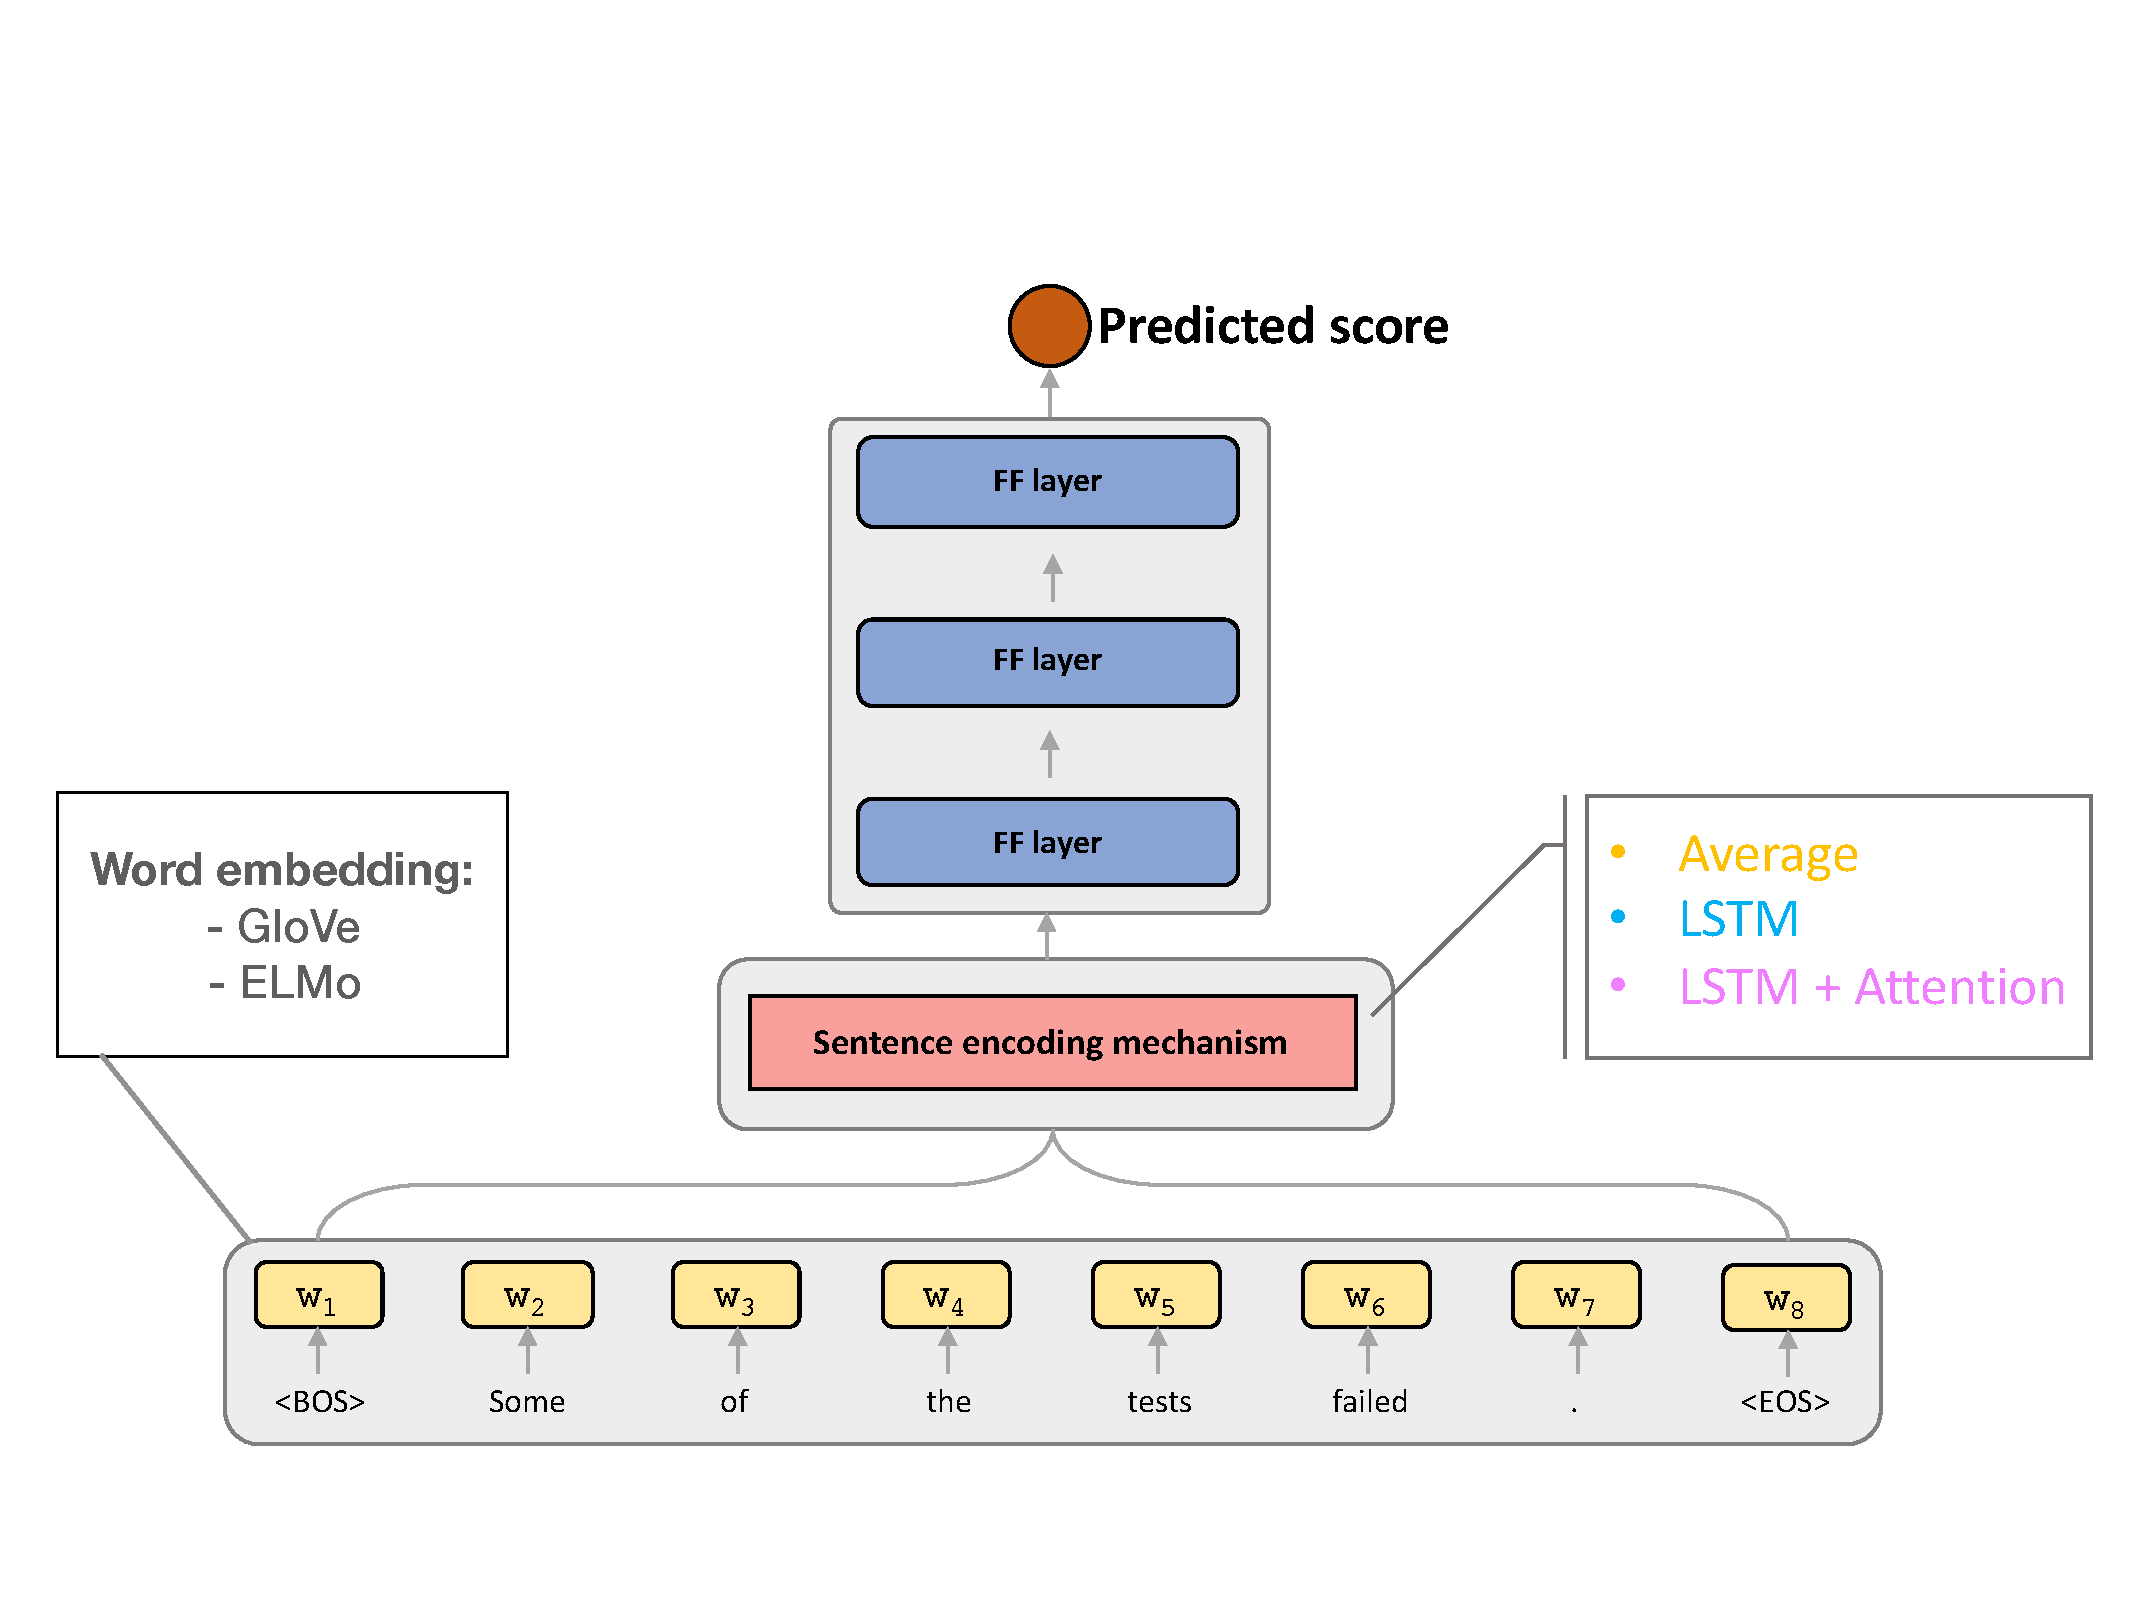
\includegraphics[width=.5\textwidth]{images/modelarchitecture}
	\caption{Model architecture.}
	\label{fig:modelarchitecture}
\end{figure}

\subsection{Word embedding model}

\jd{GLoVe vs ELMo descriptionn (and BERT if we're using it?)}

\subsection{Sentence embedding model}

\jd{meann vs LSTM vs LSTM plus attention}

\jd{also mention here: manipulation of whether or not context was included in the sentence embedding (in which case, i suppose, it's no longer strictly a sentence embedding)}

\section{Model evaluation}

\subsection{Model performance}

\jd{Main points: 1. asymptotic performance very similar across ELMo based models (which are generally better than the GLoVe models). 2. Averaging is dumb (because it gets rid of signal). 3. Whether you use LSTM with or without attention doesn't matter for asymptotic performance, but it learns more quickly with attention. 4. Whether or not context is used doesn't matter for the best performing model. refer to \figref{fig:modelperformance}, which may need to be remade with BERT results (but only if they're better)}

\begin{figure}
	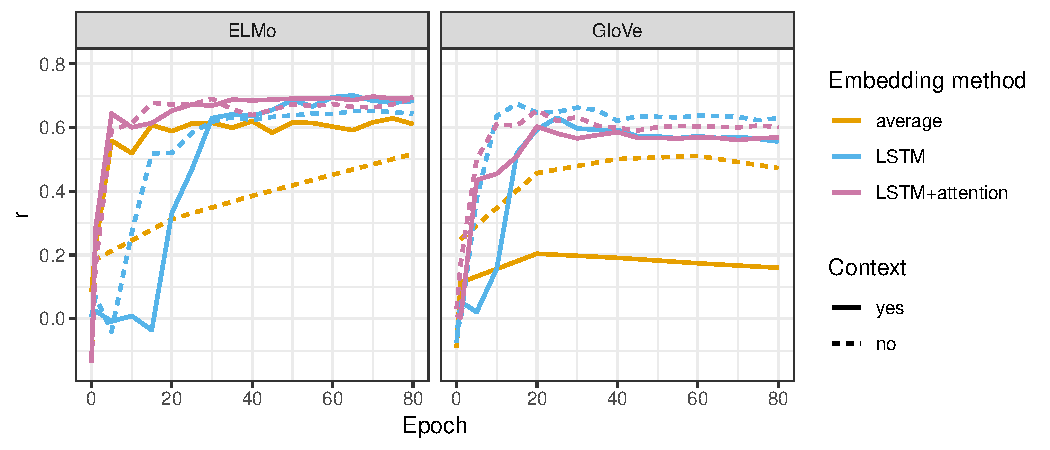
\includegraphics[width=.5\textwidth]{../models/graphs/model_performance_epoch80_6}
	\caption{Correlation of each model's predictions with empirical means, by training epoch.}
	\label{fig:modelperformance}
\end{figure}

\subsection{Re-analysis of original dataset with neural model indicator}

\jd{Main point: Including the best neural model predictions (in the talk that was ELMo - LSTM + attention - with context) as indicator in original regression model makes all other effects disappear}
 
\jd{refer back to the table from the dataset section to make the point that all effects disappear}

\jd{include scatterplots like on slide 105 to make point that variance explained is very similar}

While this is an impressive result, it is not clear whether the neural model captures the same amount of variance as the hand-mined features because it's encoding the same information, or for a different reason. We next provide a small qualitative analysis to address this question.

\subsection{Qualitative model evaluation}


\begin{figure}
	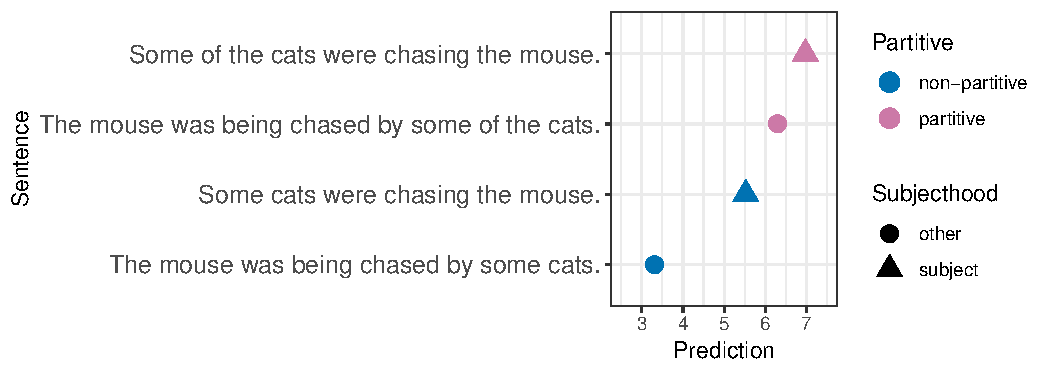
\includegraphics[width=.5\textwidth]{../models/graphs/qualitative_prediction_means_partsubj}
	\caption{Model prediction for artificial dataset of four sentences that are minimal variations of each other where partitive and subjecthood are crossed.}
	\label{fig:modelqualitative}
\end{figure}

\section{General discussion}

XXX

\bibliographystyle{apacite}

\setlength{\bibleftmargin}{.125in}
\setlength{\bibindent}{-\bibleftmargin}

\bibliography{bibs.bib}
%
%
%\section{General Formatting Instructions}
%
%The entire content of a paper (including figures, references, and anything else) can be no longer than six pages in the \textbf{initial submission}. In the \textbf{final submission}, the text of the paper, including an author line, must fit on six pages. Up to one additional page can be used for acknowledgements and references.
%
%The text of the paper should be formatted in two columns with an
%overall width of 7 inches (17.8 cm) and length of 9.25 inches (23.5
%cm), with 0.25 inches between the columns. Leave two line spaces
%between the last author listed and the text of the paper; the text of
%the paper (starting with the abstract) should begin no less than 2.75 inches below the top of the
%page. The left margin should be 0.75 inches and the top margin should
%be 1 inch.  \textbf{The right and bottom margins will depend on
%  whether you use U.S. letter or A4 paper, so you must be sure to
%  measure the width of the printed text.} Use 10~point Times Roman
%with 12~point vertical spacing, unless otherwise specified.
%
%The title should be in 14~point bold font, centered. The title should
%be formatted with initial caps (the first letter of content words
%capitalized and the rest lower case). In the initial submission, the
%phrase ``Anonymous CogSci submission'' should appear below the title,
%centered, in 11~point bold font.  In the final submission, each
%author's name should appear on a separate line, 11~point bold, and
%centered, with the author's email address in parentheses. Under each
%author's name list the author's affiliation and postal address in
%ordinary 10~point type.
%
%Indent the first line of each paragraph by 1/8~inch (except for the
%first paragraph of a new section). Do not add extra vertical space
%between paragraphs.
%
%
%\section{Formalities, Footnotes, and Floats}
%
%Use standard APA citation format. Citations within the text should
%include the author's last name and year. If the authors' names are
%included in the sentence, place only the year in parentheses, as in
%\citeA{NewellSimon1972a}, but otherwise place the entire reference in
%parentheses with the authors and year separated by a comma
%\cite{NewellSimon1972a}. List multiple references alphabetically and
%separate them by semicolons
%\cite{ChalnickBillman1988a,NewellSimon1972a}. Use the
%``et~al.'' construction only after listing all the authors to a
%publication in an earlier reference and for citations with four or
%more authors.
%
%
%\subsection{Footnotes}
%
%Indicate footnotes with a number\footnote{Sample of the first
%footnote.} in the text. Place the footnotes in 9~point font at the
%bottom of the column on which they appear. Precede the footnote block
%with a horizontal rule.\footnote{Sample of the second footnote.}
%
%
%\subsection{Tables}
%
%Number tables consecutively. Place the table number and title (in
%10~point) above the table with one line space above the caption and
%one line space below it, as in Table~\ref{sample-table}. You may float
%tables to the top or bottom of a column, and you may set wide tables across
%both columns.
%
%\begin{table}[H]
%\begin{center} 
%\caption{Sample table title.} 
%\label{sample-table} 
%\vskip 0.12in
%\begin{tabular}{ll} 
%\hline
%Error type    &  Example \\
%\hline
%Take smaller        &   63 - 44 = 21 \\
%Always borrow~~~~   &   96 - 42 = 34 \\
%0 - N = N           &   70 - 47 = 37 \\
%0 - N = 0           &   70 - 47 = 30 \\
%\hline
%\end{tabular} 
%\end{center} 
%\end{table}
%
%
%\subsection{Figures}
%
%All artwork must be very dark for purposes of reproduction and should
%not be hand drawn. Number figures sequentially, placing the figure
%number and caption, in 10~point, after the figure with one line space
%above the caption and one line space below it, as in
%Figure~\ref{sample-figure}. If necessary, leave extra white space at
%the bottom of the page to avoid splitting the figure and figure
%caption. You may float figures to the top or bottom of a column, and
%you may set wide figures across both columns.
%
%\begin{figure}[H]
%\begin{center}
%\fbox{CoGNiTiVe ScIeNcE}
%\end{center}
%\caption{This is a figure.} 
%\label{sample-figure}
%\end{figure}
%
%
%\section{Acknowledgments}
%
%In the \textbf{initial submission}, please \textbf{do not include
%  acknowledgements}, to preserve anonymity.  In the \textbf{final submission},
%place acknowledgments (including funding information) in a section \textbf{at
%the end of the paper}.
%
%
%\section{References Instructions}
%
%Follow the APA Publication Manual for citation format, both within the
%text and in the reference list, with the following exceptions: (a) do
%not cite the page numbers of any book, including chapters in edited
%volumes; (b) use the same format for unpublished references as for
%published ones. Alphabetize references by the surnames of the authors,
%with single author entries preceding multiple author entries. Order
%references by the same authors by the year of publication, with the
%earliest first.
%
%Use a first level section heading, ``{\bf References}'', as shown
%below. Use a hanging indent style, with the first line of the
%reference flush against the left margin and subsequent lines indented
%by 1/8~inch. Below are example references for a conference paper, book
%chapter, journal article, dissertation, book, technical report, and
%edited volume, respectively.
%
%\nocite{ChalnickBillman1988a}
%\nocite{Feigenbaum1963a}
%\nocite{Hill1983a}
%\nocite{OhlssonLangley1985a}
%% \nocite{Lewis1978a}
%\nocite{Matlock2001}
%\nocite{NewellSimon1972a}
%\nocite{ShragerLangley1990a}





\end{document}